\documentclass{beamer}

\usepackage{pgfpages}
% Note rendering settings
% \setbeameroption{hide notes} % Default
% \setbeameroption{show notes}
% \setbeameroption{show only notes}
% \setbeameroption{show notes on second screen}

% Maths
\usepackage{mathabx}
\usepackage{mathtools}

% Support for sane handling of values with SI units
\usepackage{siunitx}

% Algorithms using algorithmicx package (with its algpseudocode command set)
\usepackage{algpseudocode}

% Code listings
\usepackage{listings}
\usepackage{lstautogobble}
\lstset{
		basicstyle=\small,
		breaklines=true,
		autogobble=true,
		postbreak=\mbox{$\drsh$},
}

% Date management
\usepackage{datetime2}
\DTMsavedate{presentation}{2022-12-07}

% BibLaTeX
\usepackage[
  style=alphabetic,
  backend=biber, % Default backend, just listed for completness
  sorting=ynt % Sort by year, name, title
]{biblatex}
\addbibresource{references.bib}
\nocite{*}

% A more modern (and less beamer-y) theme
\usetheme{metropolis}

% \metroset{sectionpage=simple}
% Optional light gray fill behind block environments such as \theorem
\metroset{block=fill}

\title{Punchscan}
\subtitle{Paper-based voting with E2E auditing capabilities}
\author{Michael Senn}
\institute{Faculty of Science, University of Bern}
\date{\DTMusedate{presentation}}

\begin{document}

\maketitle

\section{Motivation}

\begin{frame}{Motivation}
	To provide a voting system, where:
	\begin{itemize}
		\item The vote is managed by a central election authority
		\item And voters get a paper-based receipt
		\item Which does not allow votes to be bought nor coerced
		\item Yet allows them to verify their votes are cast-as-intended
		\item And auditors provide resilience against a malicious EA
	\end{itemize}
\end{frame}

\section{Ballot layout}

\begin{frame}{Ballot layout}
	\begin{itemize}
		\item Ballot consists of two pages, stacked on top of each other
		\item Both pages have serial number identifying ballot
	\end{itemize}
	\begin{figure}
		\centering
		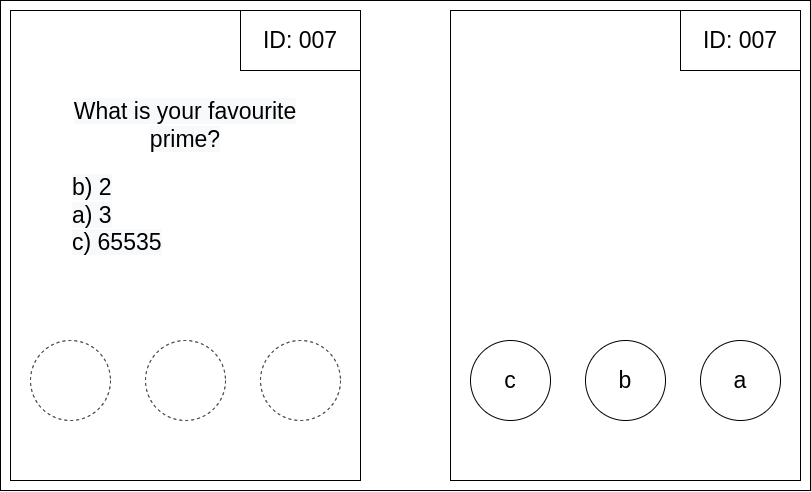
\includegraphics[width=0.65\textwidth]{../resources/high_level_ballot.drawio.png}
		\caption{Top (left) and bottom (right) halves of ballot}
	\end{figure}
\end{frame}

\begin{frame}{Ballot layout: Top page}
	\begin{itemize}
		\item Top page has question and answers, mapped to symbols (here: letters)
		\item This mapping is randomized per ballot
		\item Circular cutouts allow seeing bottom page
	\end{itemize}
	\begin{figure}
		\centering
		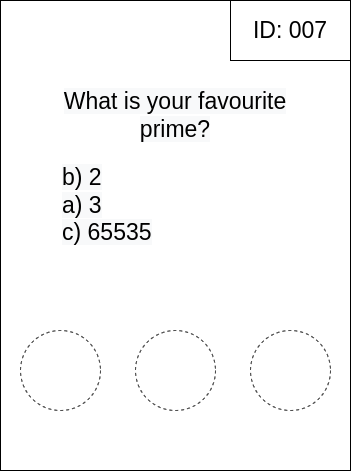
\includegraphics[width=0.3\textwidth]{../resources/high_level_ballot_top.drawio.png}
		\caption{Top half of ballot}
	\end{figure}
\end{frame}

\begin{frame}{Ballot layout: Bottom page}
	\begin{itemize}
		\item Bottom page has answer symbols (here: letters)
		\item Order of these is randomized per ballot
		\item Symbols can be seen through cutouts in top page
	\end{itemize}
	\begin{figure}
		\centering
		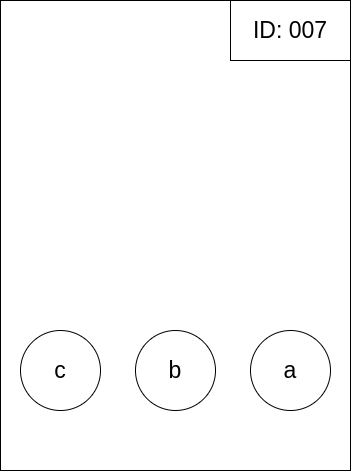
\includegraphics[width=0.3\textwidth]{../resources/high_level_ballot_bottom.drawio.png}
		\caption{Bottom half of ballot}
	\end{figure}
\end{frame}

\section{Voting process}

\begin{frame}{Voting process: Voting}
	\begin{itemize}
		\item Voter receives ballot, both pages stacked atop each other
		\item Voter marks their choice using a dauber (huge highlighter)
		\item This leaves stain on both top and bottom page
	\end{itemize}
	\begin{figure}
		\centering
		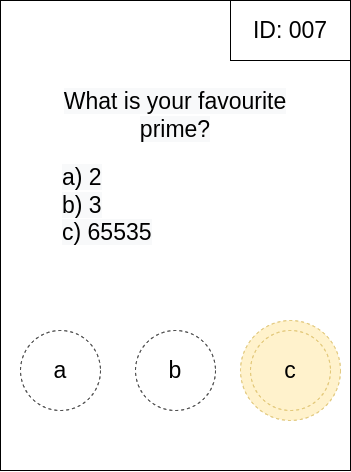
\includegraphics[width=0.3\textwidth]{../resources/high_level_ballot_voted.drawio.png}
		\caption{Ballot after voting}
	\end{figure}
\end{frame}

\begin{frame}{Voting process: Scanning}
	\begin{itemize}
		\item Voter destroys one half of the ballot
		\item Other half gets scanned, and kept by voter as receipt
		\item Unable to learn vote by looking at one half only
		\item But: What to do in tally phase?
	\end{itemize}
	\begin{figure}
		\centering
		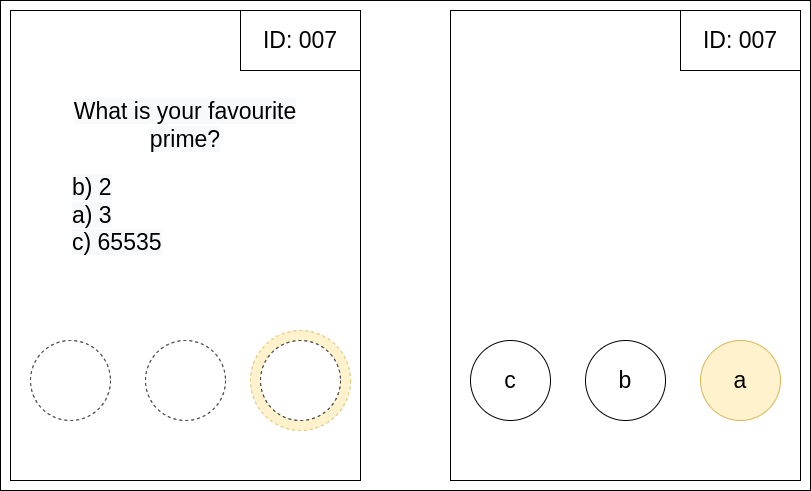
\includegraphics[width=0.65\textwidth]{../resources/high_level_ballot_voted_split.drawio.png}
		\caption{Top (left) and bottom (right) halves of ballot after voting}
	\end{figure}
\end{frame}


\section{References}

\begin{frame}[allowframebreaks]
	\frametitle{References}
	\printbibliography
\end{frame}


% \begin{frame}{Non-Goal}
% 		\begin{itemize}
% 				\item Keys only added during initialization
% 						\begin{itemize}
% 								\item Late addition can be done, but not
% 										described in paper
% 						\end{itemize}
% 				\item No updates or deletion of keys
% 				\item Fully in-memory
% 				\item Less tight / rigorous bounds on false-positive error rate
% 						than e.g. Bloom filter
% 		\end{itemize}
% \end{frame}
% 
% \section{Data structure layout}
% 
% \begin{frame}{How to efficiently encode a trie?}
% 		\begin{columns}
% 				\column{0.3\textwidth}
% 				\begin{figure}
% 						\centering
% 						\includegraphics[width=\textwidth]{resources/trie.png}
% 						\caption{Trie \autocite{booyabazookaTrieExampleSvg}}
% 				\end{figure}
% 				\column{0.7\textwidth}
% 				\begin{itemize}
% 						\item Assume trie of bytes, 64bit architecture
% 						\item Naive approach: For each edge, store its value and
% 								pointers to child node
% 						\item Then $k \cdot (8 + 64)$ bit for $k$-child node
% 						\item Hugely inefficient. Encoding \qty{1}{\byte} costs
% 								\qty{9}{\byte}!
% 						\item Enter LOUDS: space-efficient level-order encoding
% 								of tries \autocite{jacobsonSpaceefficientStaticTrees1989}
% 				\end{itemize}
% 		\end{columns}
% \end{frame}
% 
% \begin{frame}{FST: Fast succinct tries}
% 		\begin{block}{Observation}
% 						Upper levels of tries have many edges, lower levels
% 						have few. Yet most accesses are to nodes of upper level.
% 		\end{block}
% 
% 		\begin{itemize}
% 				\item FST: Trie of keys, encoded with two variants of LOUDS encoding
% 				\item LOUDS-DENSE for upper levels: Optimized for fast lookup
% 				\item LOUDS-SPARSE  for lower levels: Optimized for compact storage
% 		\end{itemize}
% \end{frame}
% 
% \begin{frame}{LOUDS-SPARSE}
% 		\begin{itemize}
% 				\item Three byte sequences: S-Labels, S-HasChild, S-LOUDS
% 						\begin{itemize}
% 								\item S-Labels: List of edges
% 								\item S-HasChild: 1 IFF edge has FST sub-trie
% 								\item S-LOUDS: 1 IFF edge is first in node
% 						\end{itemize}
% 				\item Plus byte sequence of associated values
% 				\item Assume we want to store keys `f', `fa', `s'.
% 		\end{itemize}
% \end{frame}
% 
% \begin{frame}{LOUDS-SPARSE: Example}
% 		\begin{columns}
% 				\column{0.4\textwidth}
% 				\begin{figure}
% 						\centering
% 						\includegraphics[width=\textwidth]{resources/louds_trie}
% 						\caption{Example FST}
% 				\end{figure}
% 				\column{0.6\textwidth}
% 				\begin{figure}
% 						\centering
% 						\includegraphics[width=\textwidth]{resources/louds_sparse}
% 						\caption{And its LOUDS-SPARSE encoding}
% 				\end{figure}
% 		\end{columns}
% \end{frame}
% 
% \begin{frame}{SURF}
% 		\begin{itemize}
% 				\item FST with top $k$ levels as LOUDS-DENSE, rest as
% 						LOUDS-SPARSE
% 				\item Truncate keys as much as possible while still allowing
% 						disambiguation
% 				\item Optionally use $n$ additional bits to store additional
% 						information about keys
% 						\begin{itemize}
% 								\item Bits of actual key: Good for point and
% 										range queries, no tight bound on error
% 										probability
% 								\item Bits of hashed key: Good only for point
% 										queries, tight bound on error
% 										probability
% 						\end{itemize}
% 		\end{itemize}
% \end{frame}
% 
% \begin{frame}{SURF: Base, Hash, Real}
% 		\begin{figure}
% 				\centering
% 				\includegraphics[width=\textwidth]{resources/surf}
% 				\caption{SURF variants \autocite{zhangSuRFPracticalRange2018}}
% 		\end{figure}
% \end{frame}
% 
% \section{Operations}
% 
% \subsection{Lookup operations}
% 
% \begin{frame}{Lookup operations}
% 		\begin{itemize}
% 				\item Lookup operations can be implemented as combination of
% 						$\operatorname{rank}$ and $\operatorname{select}$
% 						queries on LOUDS-encoded datastructure.
% 				\item $\operatorname{rank}_b(x)$: Number of bits with value $b$
% 						up to position $x$
% 				\item $\operatorname{select}_b(x)$: Position of $x$-th bit with value $b$
% 				\item $B = 100010110$, $\operatorname{rank}_0(5) = 4$,
% 						$\operatorname{select}_1(2) = 4$
% 				\item Constant-time with use of lookup-tables: Cache rank and
% 						select every $x$ bits, only count inbetween
% 		\end{itemize}
% \end{frame}
% 
% \begin{frame}{Lookup operation: Example of point lookup for `toy'}
% 		\begin{itemize}
% 				\item Lookup of key `toy'
% 				\item Example with LOUDS-SPARSE, as bitmap-heavy LOUDS-DENSE not
% 						very human-friendly
% 				\item Given node starting at index $p$, find index of its $k$-th child:
% 						\[
% 								\operatorname{select}_1(S\text{-}LOUDS, \operatorname{rank}_1(S\text{-}HasChild, p+k) + 1)
% 						\]
% 		\end{itemize}
% \end{frame}
% 
% \begin{frame}{Lookup operation: Example of point lookup for `toy'}
% 		\begin{figure}
% 				\centering
% 				\includegraphics[width=\textwidth]{resources/surf_point_lookup_1}
% 				\caption{Point lookup for `toy'}
% 		\end{figure}
% \end{frame}
% 
% \begin{frame}{Lookup operation: Example of point lookup for `toy'}
% 		\begin{figure}
% 				\centering
% 				\includegraphics[width=\textwidth]{resources/surf_point_lookup_2}
% 				\caption{Point lookup for `toy'}
% 		\end{figure}
% \end{frame}
% 
% \begin{frame}{Lookup operation: Example of point lookup for `toy'}
% 		\begin{figure}
% 				\centering
% 				\includegraphics[width=\textwidth]{resources/surf_point_lookup_3}
% 				\caption{Point lookup for `toy'}
% 		\end{figure}
% \end{frame}
% 
% \section{Performance}
% 
% % Not required according to newest documents
% 
% \begin{frame}{Performance evaluation}
% 		\textbf{Some high-level non-quantitative results from the SuRF paper}
% 		\begin{itemize}
% 				\item SuRF has higher false-positive rate than bloom
% 				\item Hence outperformed (in RocksDB) by bloom filter for point queries
% 				\item But allows to speed up range query throughput by \qty{50}{\percent}
% 		\end{itemize}
% \end{frame}
% 
% \section{Summary \& QA}
% 
% \begin{frame}{Summary}
% 		\begin{itemize}
% 				\item SuRF: Data structure for probabilistic point and range
% 						membership queries
% 				\item FST: Succinct encoding of truncated tries
% 				\item LOUDS-DS: Encoding of tries, made for fast traversal of
% 						upper levels and compact storage of lower levels
% 		\end{itemize}
% \end{frame}
% 
% \appendix
% \section{\appendixname}
% 
% \begin{frame}{LOUDS-DENSE}
% 		\begin{itemize}
% 				\item Three bitmaps: D-Labels, D-HasChild, D-IsPrefixKey
% 						\begin{itemize}
% 								\item D-Labels: Set bits corresponding to edges
% 								\item D-HasChild: Set bits if corresponding edge has FST sub-trie
% 								\item D-IsPrefixKey: Set bit if path up to node is a key
% 						\end{itemize}
% 				\item $\qty{513}{\bit}$ per node
% 				\item Plus byte sequence of associated values
% 		\end{itemize}
% \end{frame}
% 
% \begin{frame}{LOUDS-DENSE: Example}
% 		\begin{columns}
% 				\column{0.35\textwidth}
% 				\begin{figure}
% 						\centering
% 						\includegraphics[width=\textwidth]{resources/louds_trie}
% 						\caption{Example FST}
% 				\end{figure}
% 				\column{0.65\textwidth}
% 				\begin{figure}
% 						\centering
% 						\includegraphics[width=\textwidth]{resources/louds_dense}
% 						\caption{And its LOUDS-DENSE encoding}
% 				\end{figure}
% 		\end{columns}
% \end{frame}
% 
% 
% \subsection{Initializing SuRF}
% 
% \begin{frame}{Initializing SuRF}
% 		\begin{itemize}
% 				\item \textbf{Goal} Given set of sorted keys, turn it into SuRF
% 						data structure (i.e. LOUDS-encoded FST)
% 				\item Not specified by paper
% 				\item Depth-first: Process keys one by one
% 						\begin{itemize}
% 								\item Fairly straight-forward for generic tries
% 								\item But LOUDS is a level-order encoding. No
% 										clue where to place nodes in memory
% 										before we encoded all nodes before it.
% 						\end{itemize}
% 
% 				\item Breadth-firsth: Process keys in parallel, byte by byte.
% 						\begin{itemize}
% 								\item Allows to encode all nodes of one level
% 										before moving on to the next
% 								\item But requires keeping track of which keys
% 										go where
% 						\end{itemize}
% 		\end{itemize}
% \end{frame}
% 
% \begin{frame}{Initializing SuRF: Breadth-first}
% 		\begin{figure}
% 				\centering
% 				\includegraphics[width=\textwidth]{resources/initializing_surf_1}
% 				\caption{Initializing SuRF}
% 		\end{figure}
% \end{frame}
% 
% \begin{frame}{Initializing SuRF: Breadth-first}
% 		\begin{figure}
% 				\centering
% 				\includegraphics[width=0.9\textwidth]{resources/initializing_surf_2}
% 				\caption{Initializing SuRF}
% 		\end{figure}
% 
% 		\note[item]{Edge for `f' is set (D-Labels respectively S-Labels)}
% 		\note[item]{There are keys left which pass through that node, so it has
% 		an FST sub-component there. (D-HasChild respectively S-HasChild)}
% 		\note[item]{A key ends on that node. (D-IsPrefixKey)}
% 		\note[item]{Have left out storing of values for brevity}
% 		\note[item]{Edge for `s' is set}
% 		\note[item]{No more keys along that path, so no FST sub-component}
% \end{frame}
% 
% \begin{frame}{Initializing SuRF: Breadth-first}
% 		\begin{figure}
% 				\centering
% 				\includegraphics[width=0.7\textwidth]{resources/initializing_surf_3}
% 				\caption{Initializing SuRF}
% 		\end{figure}
% \end{frame}
% 
% \begin{frame}{Initializing SuRF: Breadth-first}
% 		\begin{figure}
% 				\centering
% 				\includegraphics[height=0.6\textwidth]{resources/initializing_surf_4}
% 				\caption{Initializing SuRF}
% 		\end{figure}
% \end{frame}
% 
% \begin{frame}{Initializing SuRF: Breadth-first}
% 		\begin{figure}
% 				\centering
% 				\includegraphics[width=0.6\textwidth]{resources/initializing_surf_5}
% 				\caption{Initializing SuRF}
% 		\end{figure}
% 
% 		\note[item]{Until we finally have initialized the whole tree}
% 		\note[item]{Note that some details left out: Handling change from
% 		LOUDS-DENSE to LOUDS-SPARSE, values, ...}
% 		\note[item]{Possible that added complexity outweights cost of copying
% 		memory, so depth-first might be faster}
% \end{frame}


\end{document}
